\chapter{Contents of \texttt{ueathesis.sty}}

\begin{synopsis}
\noindent NOTE: The compilation of this document was done with the \verb|ueathesis.cls| file, with the chapter heading option set to [Center aligned (chapternumber \verb|\\| chaptername \verb|\\| hline)]. However, \verb|ueathesis.sty| is also compatible with the document class \verb|book|, which removes this synopsis environment and the fancy chapter headings.
\end{synopsis}

Numbers refer to sections of the style file. Bulleted lists refer to options; one bullet indicates a command to be commented in or out, more than two indicates an either/or choice. A \textbf{bold} item in a bulleted list indicates the default option, used in compilation of this document.

All options comply with UEA Thesis guidelines.

\begin{enumerate}[\bf 1]
\item Initial packages

\item Layout options
\begin{enumerate}[2.1]
\item Margins
\begin{itemize}
\item Two sided options
\item \textbf{One sided options}
\end{itemize}
\item Line spacing
\begin{itemize}
\item One half spaced
\item \textbf{Double spaced}
\end{itemize}
\item Paragraph indentation and spacing
\begin{itemize}
\item Indent, no skip
\item \textbf{No indent, skip}
\end{itemize}
\item Ragged edges
\begin{itemize}
\item Ragged right edge \textbf{on} or off (right justification)
\end{itemize}
\item Font choices
\begin{itemize}
\item \textbf{Default (Computer Modern Roman)}
\item Charter
\item Fourier
\item Helvetica
\item Latin Modern Roman
\item Palatino
\item Times
\end{itemize}
\item Fancy heading options
\begin{itemize}
\item Two sided options
\item \textbf{One sided options}
\end{itemize}
\end{enumerate}

\item Machinery for environments and numbering
\begin{enumerate}[3.1]
\item \verb|hyperref| display options
\begin{itemize}
\item Coloured frames, black text
\item \textbf{No frames, coloured text}
\item No frames, black text
\end{itemize}
\item Equation numbering
\begin{itemize}
\item Equation numbering \textbf{by section} or by chapter
\end{itemize}
\item Figure and table numbering
\begin{itemize}
\item Figure numbering \textbf{by section} or by chapter
\item Table numbering by section or \textbf{by chapter}
\end{itemize}
\item Theorem environments and numbering
\begin{itemize}
\item \textbf{Full name environments}
\item Abbreviated environments
\end{itemize}
\end{enumerate}

\item Tabular and drawing options
\begin{enumerate}[4.1]
\item Table packages and spacing
\begin{itemize}
\item Table row stretching to avoid clashes with \verb|\hline| \textbf{on} or off
\end{itemize}
\item TikZ packages and libraries
\item Some nice TikZ arrows
\end{enumerate}

\item Custom commands and macros
\begin{enumerate}[5.1]
\item Todo notes
\item New mathematical operators/indicators
\item Math fonts
\item Labelled arrows
\item Advanced bracketing support
\item Mathematical diacritics
\item Vectors and matrices
\item Calculus
\item SI unit handling
\item Properly typeset mathematical constants
\item Proper superscripting and subscripting
\item Miscellaneous
\end{enumerate}
\end{enumerate}


\chapter{Nice things in \texttt{ueathesis.sty}}

\begin{synopsis}
\noindent This chapter contains a user guide to all of the nifty features included in \verb|ueathesis.sty|.
\end{synopsis}

\section{Nice things for mathematicians}

\subsection{Easy vectors}

Tired of typing out vectors? You can use these nice predefined commands. If you don't like any of these as the abbreviated commands for vectors, then you can change them in the \verb|ueathesis.sty| file.

\begin{verbatim}
\[\onetwo{a_1}{a_2}\twotwo{1}{0}{0}{1} = \onetwo{a_1}{a_2}\]
\end{verbatim}

\[\onetwo{a_1}{a_2}\twotwo{1}{0}{0}{1} = \onetwo{a_1}{a_2}\]

\begin{spverbatim}
\[\onethree{a_1}{a_2}{a_3}\threethree{1}{0}{0}{0}{1}{0}{0}{0}{1} = \onethree{a_1}{a_2}{a_3}\]
\end{spverbatim}

\[\onethree{a_1}{a_2}{a_3}\threethree{1}{0}{0}{0}{1}{0}{0}{0}{1} = \onethree{a_1}{a_2}{a_3}\]

\begin{spverbatim}
\[\onen{a_1}{a_2}{a_n}\nbyn{1}{0}{0}{0}{1}{0}{0}{0}{1} = \onen{a_1}{a_2}{a_n}\]
\end{spverbatim}

\[\onen{a_1}{a_2}{a_n}\nbyn{1}{0}{0}{0}{1}{0}{0}{0}{1} = \onen{a_1}{a_2}{a_n}\]

\subsection{Todo notes}{\label{sec:todo}}

The \verb|todonotes| package allows you to make quick notes in your \LaTeX{} document to keep track of what needs to be done. We have provided four different types, using four different colours:
\begin{itemize}
\item \verb|\unsure{What?}|, in red
\item \verb|\change{huh?}|, in blue
\item \verb|\info{Eh?}|, in yellow
\item \verb|\improvement{Que?}|, in green
\end{itemize}

You can add more, or change the names/displayed colours of the commands by tinkering with \verb|ueathesis.sty|. By including \verb|inline| as an optional argument (so, for instance, \verb|\info[inline]{ARGH!}|), the todo note will split the text, making it more noticeable. These commands have been used in the dummy text below; the verbatim for this is given in \autoref{app:verb}.

Nulla id metus justo. Ut imperdiet enim vel tellus dignissim\unsure{What?}, nec sollicitudin quam commodo. Orci varius natoque penatibus et magnis\change{huh?} dis parturient montes, nascetur ridiculus mus. Praesent vel rutrum urna. Curabitur\info{Eh?} in purus interdum, mollis arcu non, aliquet metus. Donec dapibus est feugiat ex faucibus, sed interdum massa molestie. Nam eu metus \info[inline]{ARGH!} pellentesque, finibus velit in, mattis tellus. Etiam euismod, arcu nec sodales pellentesque, justo mi euismod felis, sed volutpat tortor lacus eget justo. Suspendisse quis lobortis lectus\improvement{Que?}. Ut eleifend aliquet varius. Suspendisse vulputate neque vel nibh dignissim ullamcorper. 

Want to know exactly where you've left a to do note? You can include a list of todonotes by using the command \verb|\listoftodos|; this will then usefully list your to do notes. We have done this at the end of the body text, just before the bibliography.

\begin{remark} To do notes added by the \verb|todonotes| package appears on printed versions; so make sure these are removed from your thesis prior to submission!
\end{remark}

\subsection{The Joy Of TikZ: examples for all!}
The \verb|TikZ| package is a powerful way of inserting images/graphs/sketches into your thesis. The package allows you to create a \verb|tikzpicture|, wherein you can code lines, curves, circles, grids and much more using \TeX{} code. While this will likely be used in quite a niche way for most theses, we've included some examples here that demonstrate different commands within a \verb|TikZ| environment that can be used.

Note that the authors are still learning TikZ; and the code in the style file may not be the best working example to display the given images.

\subsubsection{An example with code}

For example, the code
\begin{spverbatim}
\begin{figure}[ht!]
\centering
\begin{tikzpicture}
\draw[step=2cm,gray,thin] (0,0) grid (10.25,8.25);
\draw[thick,->] (0,-0.25) -- (0,8.5) node[anchor=south east] {$t_k$};
\draw[thick,->] (-0.25,0) --(10.5,0) node[anchor=north west] {$x_j$};
\draw[<->] (2.1,0.5)--(3.9,0.5) node[anchor=north east] {$\Delta x$};
\draw[<->] (0.2,2.1)--(0.2,3.9) node[anchor=north west] {$\Delta t$};
\fill[black] (6,4) circle (0.1cm) node[anchor=north west] {$u_j^k$};
\fill[black] (6,6) circle (0.1cm) node[anchor=north west] {$u_j^{k+1}$};
\fill[black] (4,4) circle (0.1cm) node[anchor=north west] {$u_{j-1}^k$};
\fill[black] (8,4) circle (0.1cm) node[anchor=north west] {$u_{j+1}^k$};
\fill[black] (6,2) circle (0.1cm) node[anchor=north west] {$u_j^{k-1}$};
\end{tikzpicture}
\caption{Mesh demonstrating numerical node structure for a finite
difference method.}
\end{figure}
\end{spverbatim}
produces \autoref{fig:mesh}.
\begin{figure}[ht!]
\centering
\begin{tikzpicture}
\draw[step=2cm,gray,thin] (0,0) grid (10.25,8.25);
\draw[thick,->] (0,-0.25) -- (0,8.5) node[anchor=south east] {$t_k$};
\draw[thick,->] (-0.25,0) --(10.5,0) node[anchor=north west] {$x_j$};
\draw[<->] (2.1,0.5)--(3.9,0.5) node[anchor=north east] {$\Delta x$};
\draw[<->] (0.2,2.1)--(0.2,3.9) node[anchor=north west] {$\Delta t$};
\fill[black] (6,4) circle (0.1cm) node[anchor=north west] {$u_j^k$};
\fill[black] (6,6) circle (0.1cm) node[anchor=north west] {$u_j^{k+1}$};
\fill[black] (4,4) circle (0.1cm) node[anchor=north west] {$u_{j-1}^k$};
\fill[black] (8,4) circle (0.1cm) node[anchor=north west] {$u_{j+1}^k$};
\fill[black] (6,2) circle (0.1cm) node[anchor=north west] {$u_j^{k-1}$};
\end{tikzpicture}
\caption{Mesh demonstrating numerical node structure for a finite
difference method.}
\label{fig:mesh}
\end{figure}
\subsubsection{Plotting functions}
You can also plot mathematical functions using TikZ. 

For example, say you wanted to plot $\sin(x)$ or $\cos(x)$, or even both.

\begin{figure}[!htbp] 
\centering
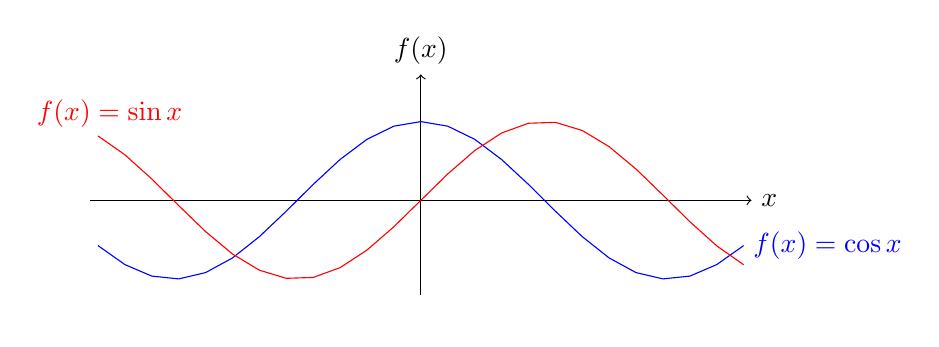
\begin{tikzpicture}[domain=-4.1:4.1]
\draw[very thin,opacity=0] (-4.1,-1.5) grid (4.1,1.5);
\draw[->] (-4.2,0) -- (4.2,0) node[right] {$x$};
\draw[->] (0,-1.2) -- (0,1.6) node[above] {$f(x)$};
% \x r means to convert ’\x’ from degrees to _r_adians:
\draw[color=blue]   plot (\x,{cos(\x r)})    node[right] {$f(x) = \cos x$};
\draw[color=red]  node[right,xshift=-5cm,yshift=1.1cm] {$f(x) = \sin x$} plot (\x,{sin(\x r)})    ;
\end{tikzpicture}
    \caption{A plot of $\sin(x)$ and $\cos(x)$ using TikZ}
    \label{fig:sincostikz1}
    \end{figure}
\autoref{fig:sincostikz1} is an example of plotting $\sin(x)$ and $\cos(x)$ together, using TikZ.   
\subsubsection{Using the \texttt{pgfplots} package}
Sometimes TikZ code isn't always appropriate for plotting certain functions. Another method for plotting functions using TikZ is to use the \verb|pgfplots| package. 

This package is also necessary for importing plots from \verb|Python| and \verb|Matlab|, using the \verb|matplotlib2tikz| and \verb|matlab2tikz| tools respectively. Both these tools will output your numerical plot into a \verb|.tex| format containing \TeX{} code in \verb|pgfplots| format. To add these to your \TeX{} document, simply add \verb|\include{plot-name.tex}| to your document, replacing ‘plot-name’ with the name of the file containing your plot.

\begin{figure}[!htbp] 
\centering
\pgfplotsset{compat=newest,width=10cm}
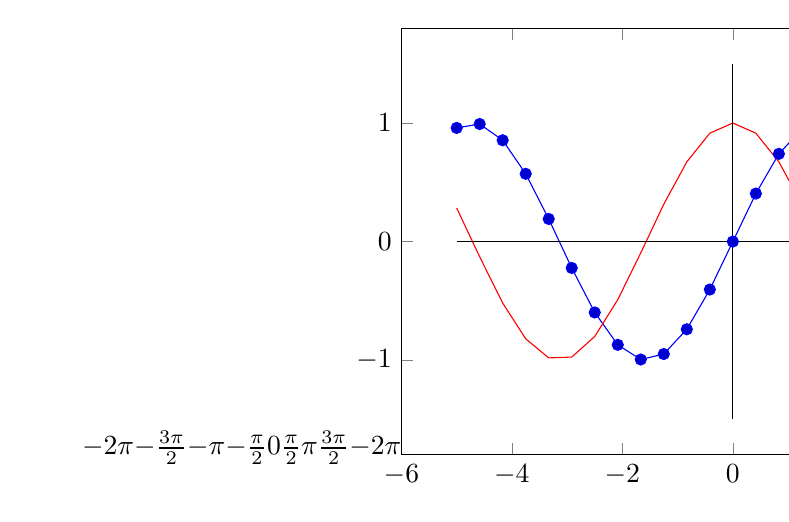
\begin{tikzpicture}
\begin{axis}
domain=(-2*pi):(2*pi),
samples=128,
no marks,
xtick={-6.28318, -4.7123889, -3.14159, -1.5708,0, 1.5708, 3.14159, 4.7123889, 6.28318},
ytick={-1,0,1},
xticklabels={$-2\pi$, $-\frac{3\pi}{2}$, $-\pi$, $-\frac{\pi}{2}$, $0$, $\frac{\pi}{2}$, $\pi$, $\frac{3\pi}{2}$, $-2\pi$},
yticklabels={-1,0,1}, 
	xmin=(-2*pi), xmax=(2*pi),
    ymin=(-1.5), ymax=(1.5)
]
\addplot {sin(\x r)}; 
\addplot [red] {cos(\x r)};
\addplot [black] {0};
\addplot +[mark=none,black] coordinates {(0, -1.5) (0, 1.5)};

    \end{axis}    \end{tikzpicture}
    \caption{A plot of $\sin(x)$ and $\cos(x)$ using \texttt{pgfplots}.}
   \label{fig:sincostikz2}
    \end{figure}

\autoref{fig:sincostikz2} shows $\sin(x)$ and $\cos(x)$ plot using \verb|pgfplots| instead of standard TikZ code. You can also plot other functions using \verb|pgfplots|.

\begin{figure}[!htbp]
\centering
\pgfplotsset{width=10cm,height=7cm}
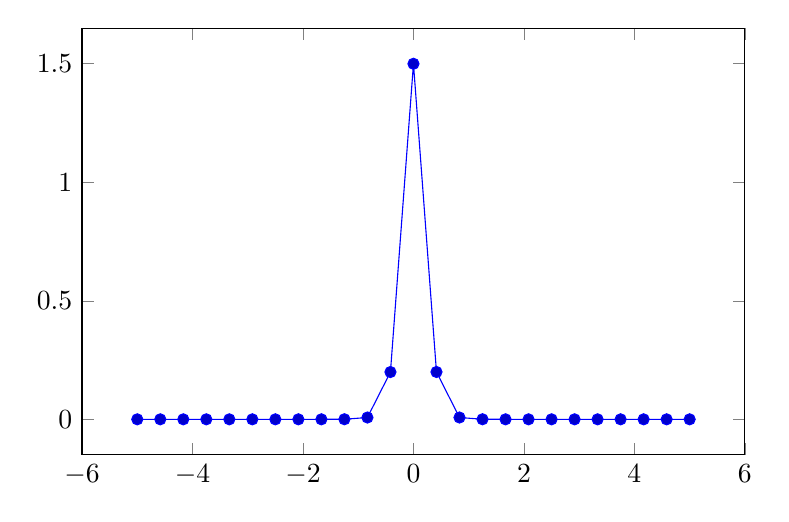
\begin{tikzpicture}
    \begin{axis}
domain=(-pi):(pi),
samples=512,
no marks, 
xticklabels={ },
yticklabels={ }, 
	xmin=(-pi), xmax=(pi),
    ymin=(-1), ymax=(2)
]
\addplot {6/((exp(4*\x) + exp(-4*\x))^(2))}; 
\draw[black,thick] (0,20)--(pi,20);
    \end{axis}
    \end{tikzpicture}
    \caption{Simple example of a solitary wave.}
    \label{fig:pgfplot1}
    \end{figure}
\autoref{fig:pgfplot1} gives an example plot of $f(x)=6\sech^2(4x)$. Note that in the TikZ code the function reads $6/(\exp(4x) + \exp(-4x))^{2}$. This is because the $\sech(x)$ and $\cosech(x)$ functions are not recognised as standard in \TeX{} (this is why we've defined them as a \verb|newcommand| in the \verb|ueathesis.sty| file).

You should also note certain properties of the domain when using \verb|pgfplots|. In \autoref{fig:pgfplot1}, the domain is defined over $[-\pi,\pi]$, as \verb|domain=(-pi):(pi)|. However, when adding lines, rectangles, nodes etc to your plot, this translates to a domain of $[0,200\pi]$. In the example, a thick, black line is drawn along the bottom of the plot, representing a bottom surface perhaps. The line is drawn between $0$ and $200\pi$ in the horizontal coordinate, to fill the whole plot. This takes a bit of getting used to, but just remember that the domain for additional nodes always starts at $0$ and will always be $100$ times larger than the domain of the plot.
\subsubsection{Graphs and directed graphs: the Joy of TikZ}

Figures \ref{fig:ladder}, \ref{fig:nicegraph}, \ref{fig:nicetikz} and \ref{fig:nicetikz2} give some nice examples of the power of TikZ in relation to drawing graphs and oriented graphs. You can find the code for these in the \verb|UEAThesisReadmeBodyText.tex| file, included with the distribution of this pdf.

\begin{figure}[ht]
\centering
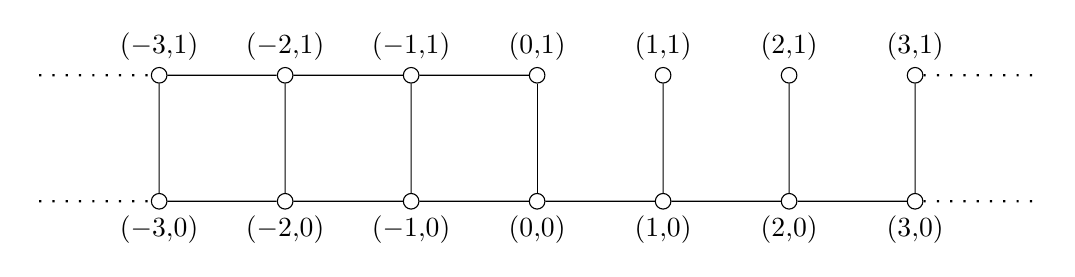
\begin{tikzpicture}[node distance=2cm,inner sep=0.7mm,scale=1.6]
\node (-a) at (-4,0.5) {};
\node (-3a) at (-3,0.5) [circle,draw,label=above:$(-3{,}1)$] {};
\node (-2a) at (-2,0.5) [circle,draw,label=above:$(-2{,}1)$] {};
\node (-1a) at (-1,0.5) [circle,draw,label=above:$(-1{,}1)$] {};
\node (0a) at (0,0.5) [circle,draw,label=above:$(0{,}1)$] {};
\node (1a) at (1,0.5) [circle,draw,label=above:$(1{,}1)$] {};
\node (2a) at (2,0.5) [circle,draw,label=above:$(2{,}1)$] {};
\node (3a) at (3,0.5) [circle,draw,label=above:$(3{,}1)$] {};
\node (+a) at (4,0.5) {};
\node (-b) at (-4,-0.5) {};
\node (-3b) at (-3,-0.5) [circle,draw,label=below:$(-3{,}0)$] {};
\node (-2b) at (-2,-0.5) [circle,draw,label=below:$(-2{,}0)$] {};
\node (-1b) at (-1,-0.5) [circle,draw,label=below:$(-1{,}0)$] {};
\node (0b) at (0,-0.5) [circle,draw,label=below:$(0{,}0)$] {};
\node (1b) at (1,-0.5) [circle,draw,label=below:$(1{,}0)$] {};
\node (2b) at (2,-0.5) [circle,draw,label=below:$(2{,}0)$] {};
\node (3b) at (3,-0.5) [circle,draw,label=below:$(3{,}0)$] {};
\node (+b) at (4,-0.5) {};
\draw (-3a) -- (-3b);
\draw (-2a) -- (-2b);
\draw (-1a) -- (-1b);
\draw (0a) -- (0b);
\draw (1a) -- (1b);
\draw (2a) -- (2b);
\draw (3a) -- (3b);
\draw [thick,loosely dotted] (-b) -- (-3b);
\draw (-3b) -- (-2b);
\draw (-2b) -- (-1b);
\draw (-1b) -- (0b);
\draw (0b) -- (1b);
\draw (1b) -- (2b);
\draw (2b) -- (3b);
\draw [thick,loosely dotted] (3b) -- (+b);
\draw [thick,loosely dotted] (-a) -- (-3a);
\draw (-3a) -- (-2a);
\draw (-2a) -- (-1a);
\draw (-1a) -- (0a);
\draw [thick,loosely dotted] (3a) -- (+a);
\end{tikzpicture}
\caption{A dangerous ladder: go up the document.}\label{fig:ladder}
\end{figure}

\begin{figure}[ht]
\centering
\begin{tikzpicture}[node distance=2cm,inner sep=0.7mm,scale=1.32]
\node (0) at (-4,0) [circle,draw,red,label=below:$v_0$] {};
\node (1) at (-3,0) [circle,draw,red,label=below:$v_1$] {};
\node (11) at (-3.25,0.25) {};
\node (111) at (-3.25,0) {};
\node (12) at (-3.25,-0.25) {};
\node (2) at (-2,0) [circle,draw,red,label=below:$v_2$] {};
\node (3) at (-1,0) [circle,draw,red,label=below:$v_{n-2}$] {};
\node (4) at (0,0) [circle,draw,red,label=below:$v_{n-1}$] {};
\node (41) at (-0.75,0.25) {};
\node (411) at (-0.75,0) {};
\node (42) at (-0.75,-0.25) {};
\node (5) at (1,0) [circle,draw,label=below:$v_n$] {};
\node (6) at (2,0) [circle,draw,label=below:$v_{n+1}$] {};
\node (7) at (3,0) [circle,draw,label=below:$v_{n+2}$] {};
\node (8) at (4,0) [circle,draw,label=below:$v_{n+3}$] {};
\node (9) at (5,0) [circle,draw,label=below:$v_{n+4}$] {};
\node (10) at (6,0) {};
\draw (0) to [out=35,in=145] (5);
\draw (1) to [out=35,in=145] (5);
\draw (2) to [out=35,in=145] (5);
\draw (3) to [out=35,in=145] (5);
\draw (4) -- (5);
\draw (0) to [out=325,in=215] (7);
\draw (1) to [out=325,in=215] (7);
\draw (2) to [out=325,in=215] (7);
\draw (3) to [out=325,in=215] (7);
\draw (4) to [out=325,in=215] (7);
\draw (5) to [out=325,in=215] (7);
\draw (6) -- (7);
\draw (0) to [out=35,in=145] (9);
\draw (1) to [out=35,in=145] (9);
\draw (2) to [out=35,in=145] (9);
\draw (3) to [out=35,in=145] (9);
\draw (4) to [out=35,in=145] (9);
\draw (5) to [out=35,in=145] (9);
\draw (6) to [out=35,in=145] (9);
\draw (7) to [out=35,in=145] (9);
\draw (8) -- (9);
\draw [thick, loosely dotted] (2) -- (3);
\draw [thick, loosely dotted] (9) -- (10);
\path [draw half paths={solid,red}{dotted,red}]  (0) -- (11);
\path [draw half paths={solid,red}{dotted,red}]  (0) -- (111);
\path [draw half paths={solid,red}{dotted,red}]  (0) -- (12);
\path [draw half paths={solid,red}{dotted,red}]  (4) -- (41);
\path [draw half paths={solid,red}{dotted,red}]  (4) -- (411);
\path [draw half paths={solid,red}{dotted,red}]  (4) -- (42);
\end{tikzpicture}
\caption{An MB-homogeneous graph with small automorphism group.}\label{fig:nicegraph}
\end{figure}


\begin{figure}[ht]
\centering
\begin{tikzpicture}[node distance=1.8cm,inner sep=0.7mm,scale=1.2]
\draw[dotted] (-5,0) rectangle (-0.4,3.5);
\draw[dotted] (0.4,0) rectangle (5,3.5);
\draw[dotted] (-3.7,1.8) rectangle (-2.3,2.2);
\draw[dotted] (-2.2,1.8) rectangle (-1.3,2.2);
\draw[dotted] (1.3,1.8) rectangle (2.7,2.2);
\draw[dotted] (2.8,1.8) rectangle (3.7,2.2);  
\node(g) at (-4.9,-0.3) {$\mc{G}$};
\node(d) at (4.9,-0.3) {$\mc{H}$};
\node(U5) at (-1.5,2) [circle,draw] {};
\node(U4) at (-2,2) [circle,draw] {};
\node(U3) at (-2.5,2) [circle,draw] {};
\node(U2) at (-3,2) [circle,draw] {};
\node(U1) at (-3.5,2) [circle,draw] {};
\node(U) at (-4,1.3) {$X_k$};
\node(Um) at (-3.2,3) {$X^\to(x_j)\cup X^\Vert(x_j)$};
\node(Un) at (-1,3) {$X^\leftarrow(x_j)$};
\node(Vm) at (1.9,3) {$(X^\to(x_j)\cup X^\Vert(x_j))f_k$};
\node(Vn) at (4.2,3) {$X^\leftarrow(x_j)f_k$};
\node(p1) at (-3,2.2) {};
\node(p2) at (-1.75,2.2) {};
\node(p3) at (2,2.2) {};
\node(p4) at (3.25,2.2) {};
\draw[dotted] (Um) -- (p1);
\draw[dotted] (Un) -- (p2);
\draw[dotted] (Vm) -- (p3);
\draw[dotted] (Vn) -- (p4);
\draw(U3) ellipse (1.8cm and 0.5cm);
\node(x) at (-2.5,0.7) [circle,draw,label=below:$x_j$] {};
\draw[middlearrow={latex}] (x) -- (U5);
\draw[middlearrow={latex}] (x) -- (U4);
%\draw[dotted] (x) -- (U3);
%\draw[dotted] (x) -- (U2);
\draw[middlearrow={latex}] (U1) -- (x);
\draw[->] (-1,1) to (1,1);
\node(fk1) at (0,0.7) {$f_{k+1}$};
\node(V1) at (1.5,2) [circle,draw] {};
\node(V1a) at (2,2) [circle,draw] {};
\node(V2) at (2.5,2) [circle,draw] {};
\node(V2a) at (3,2) [circle,draw] {};
\node(V3) at (3.5,2) [circle,draw] {};
\node(V) at (4,1.3) {$Y_k$};
\draw(V2) ellipse (1.8cm and 0.5cm);
\node(v) at (2.5,0.7) [circle,draw,label=below:$u$] {};
\draw[middlearrow={latex}] (V1) -- (v);
\draw[middlearrow={latex}] (V2) -- (v);
\draw[middlearrow={latex}] (V1a) -- (v);
\draw[middlearrow={latex}] (v) -- (V2a);
\draw[middlearrow={latex}] (v) -- (V3);
\end{tikzpicture}
\caption{$k$ even in proof of a theorem about digraphs.}\label{fig:nicetikz}
\end{figure} 


\begin{figure}[ht]
\centering
\begin{tikzpicture}[node distance=1.8cm,inner sep=0.7mm,scale=1.3]
\node(h0) at (0,0) [circle,draw] {};
\foreach \a in {1,2,...,3}{\node(h1\a) at (\a*360/3: 2cm) [circle,draw] {};}
\foreach \a in {1,2,...,17}{\node(h2\a) at (\a*360/17: 4cm) [circle,draw] {};}
\draw[thick,dotted](h0) circle (1cm);
\draw[thick,dotted](h0) circle (3cm);
\draw[thick,dotted](h0) circle (5cm);
%\draw[thick,dotted](h0) circle (7cm);
%\draw[thick,dotted] (5.5,0) to (6.5,0);
%\node(H0) at (-0.5,0.5) {$H_0$};
\node(H1) at (2.5,0) {$H_1$};
\node(H2) at (4.5,0) {$H_2$};

\draw[middlearrow={latex}] (h0) -- (h11);
\draw[middlearrow={latex}] (h12) -- (h0);

\draw[middlearrow={latex}] (h0) -- (h21);
\draw[middlearrow={latex}] (h11) -- (h21);
\draw[middlearrow={latex}] (h12) -- (h21);
\draw[middlearrow={latex}] (h13) -- (h21);

\draw[middlearrow={latex}] (h22) -- (h0);
\draw[middlearrow={latex}] (h11) -- (h22);
\draw[middlearrow={latex}] (h12) -- (h22);
\draw[middlearrow={latex}] (h13) -- (h22);

\draw[middlearrow={latex}] (h0) -- (h23);
\draw[middlearrow={latex}] (h23) -- (h11);
\draw[middlearrow={latex}] (h12) -- (h23);
\draw[middlearrow={latex}] (h13) -- (h23);

\draw[middlearrow={latex}] (h0) -- (h24);
\draw[middlearrow={latex}] (h11) -- (h24);
\draw[middlearrow={latex}] (h24) -- (h12);
\draw[middlearrow={latex}] (h13) -- (h24);

\draw[middlearrow={latex}] (h0) -- (h25);
\draw[middlearrow={latex}] (h11) -- (h25);
\draw[middlearrow={latex}] (h12) -- (h25);
\draw[middlearrow={latex}] (h25) -- (h13);

\draw[middlearrow={latex}] (h26) -- (h0);
\draw[middlearrow={latex}] (h26) -- (h11);
\draw[middlearrow={latex}] (h12) -- (h26);
\draw[middlearrow={latex}] (h13) -- (h26);

\draw[middlearrow={latex}] (h27) -- (h0);
\draw[middlearrow={latex}] (h11) -- (h27);
\draw[middlearrow={latex}] (h27) -- (h12);
\draw[middlearrow={latex}] (h13) -- (h27);

\draw[middlearrow={latex}] (h28) -- (h0);
\draw[middlearrow={latex}] (h11) -- (h28);
\draw[middlearrow={latex}] (h12) -- (h28);
\draw[middlearrow={latex}] (h28) -- (h13);

\draw[middlearrow={latex}] (h0) -- (h29);
\draw[middlearrow={latex}] (h29) -- (h11);
\draw[middlearrow={latex}] (h29) -- (h12);
\draw[middlearrow={latex}] (h13) -- (h29);

\draw[middlearrow={latex}] (h0) -- (h210);
\draw[middlearrow={latex}] (h210) -- (h11);
\draw[middlearrow={latex}] (h12) -- (h210);
\draw[middlearrow={latex}] (h210) -- (h13);

\draw[middlearrow={latex}] (h0) -- (h211);
\draw[middlearrow={latex}] (h11) -- (h211);
\draw[middlearrow={latex}] (h211) -- (h12);
\draw[middlearrow={latex}] (h211) -- (h13);

\draw[middlearrow={latex}] (h0) -- (h212);
\draw[middlearrow={latex}] (h212) -- (h11);
\draw[middlearrow={latex}] (h212) -- (h12);
\draw[middlearrow={latex}] (h212) -- (h13);

\draw[middlearrow={latex}] (h213) -- (h0);
\draw[middlearrow={latex}] (h11) -- (h213);
\draw[middlearrow={latex}] (h213) -- (h12);
\draw[middlearrow={latex}] (h213) -- (h13);

\draw[middlearrow={latex}] (h214) -- (h0);
\draw[middlearrow={latex}] (h214) -- (h11);
\draw[middlearrow={latex}] (h12) -- (h214);
\draw[middlearrow={latex}] (h214) -- (h13);

\draw[middlearrow={latex}] (h215) -- (h0);
\draw[middlearrow={latex}] (h215) -- (h11);
\draw[middlearrow={latex}] (h215) -- (h12);
\draw[middlearrow={latex}] (h13) -- (h215);

\draw[middlearrow={latex}] (h216) -- (h0);
\draw[middlearrow={latex}] (h216) -- (h11);
\draw[middlearrow={latex}] (h216) -- (h12);
\draw[middlearrow={latex}] (h216) -- (h13);

\end{tikzpicture}
\caption{Stage 2 of an infinite construction.}\label{fig:nicetikz2}
\end{figure}

\clearpage

\subsubsection{Example of a commutative diagram in $\texttt{tikz-cd}$}

This fetching diagram (\autoref{fig:snake}), drawn by Andrew Stacey of TeXample.net (reproduced here under the terms of a CC BY 2.5 licence) \cite{stacey2012snake}, illustrates the drawing power of \verb|tikz-cd|.

\begin{figure}[ht]
\centering
\begin{tikzpicture}[>=triangle 60]
  \matrix[matrix of math nodes,column sep={60pt,between origins},row
    sep={60pt,between origins},nodes={asymmetrical rectangle}] (s)
  {
    &|[name=ka]| \ker f &|[name=kb]| \ker g &|[name=kc]| \ker h \\
    %
    &|[name=A]| A' &|[name=B]| B' &|[name=C]| C' &|[name=01]| 0 \\
    %
    |[name=02]| 0 &|[name=A']| A &|[name=B']| B &|[name=C']| C \\
    %
    &|[name=ca]| \coker f &|[name=cb]| \coker g &|[name=cc]| \coker h \\
  };
  \draw[->] (ka) edge (A)
            (kb) edge (B)
            (kc) edge (C)
            (A) edge (B)
            (B) edge node[auto] {\(p\)} (C)
            (C) edge (01)
            (A) edge node[auto] {\(f\)} (A')
            (B) edge node[auto] {\(g\)} (B')
            (C) edge node[auto] {\(h\)} (C')
            (02) edge (A')
            (A') edge node[auto] {\(i\)} (B')
            (B') edge (C')
            (A') edge (ca)
            (B') edge (cb)
            (C') edge (cc)
  ;
  \draw[->,gray] (ka) edge (kb)
                 (kb) edge (kc)
                 (ca) edge (cb)
                 (cb) edge (cc)
  ;
  \draw[->,gray,rounded corners] (kc) -| node[auto,text=black,pos=.7]
    {\(\partial\)} ($(01.east)+(.5,0)$) |- ($(B)!.35!(B')$) -|
    ($(02.west)+(-.5,0)$) |- (ca);
\end{tikzpicture}
\caption{The snake lemma: go down the document.}\label{fig:snake}
\end{figure}

\subsection{Inserting figures using encapsulated postscript (.eps)}
PDF\LaTeX{} can handle three different extensions for images: \verb|.png|, \verb|.jpeg| and \verb|.pdf|. Often, you can require scalable vector graphics with no loss of quality at any zoom level. For this you can either use \verb|.pdf|, or the more traditional \verb|.eps| (which PDF\LaTeX{} cannot handle, but \LaTeX{} can). These should arguably be your default image formats, especially when using Beamer to give a presentation, as they allow you to zoom without loss of clarity. 

Many mathematical programming tools such as Maple and Matlab have the option to output images in encapsulated postscript format (\verb|.eps|). We've included a package that allows PDF\LaTeX{} to compile \verb|.eps| images. 

For this example, we'll use \verb|example_figure1.eps|, included within the documentation.

\begin{spverbatim}
\begin{figure}[ht!]
\centering
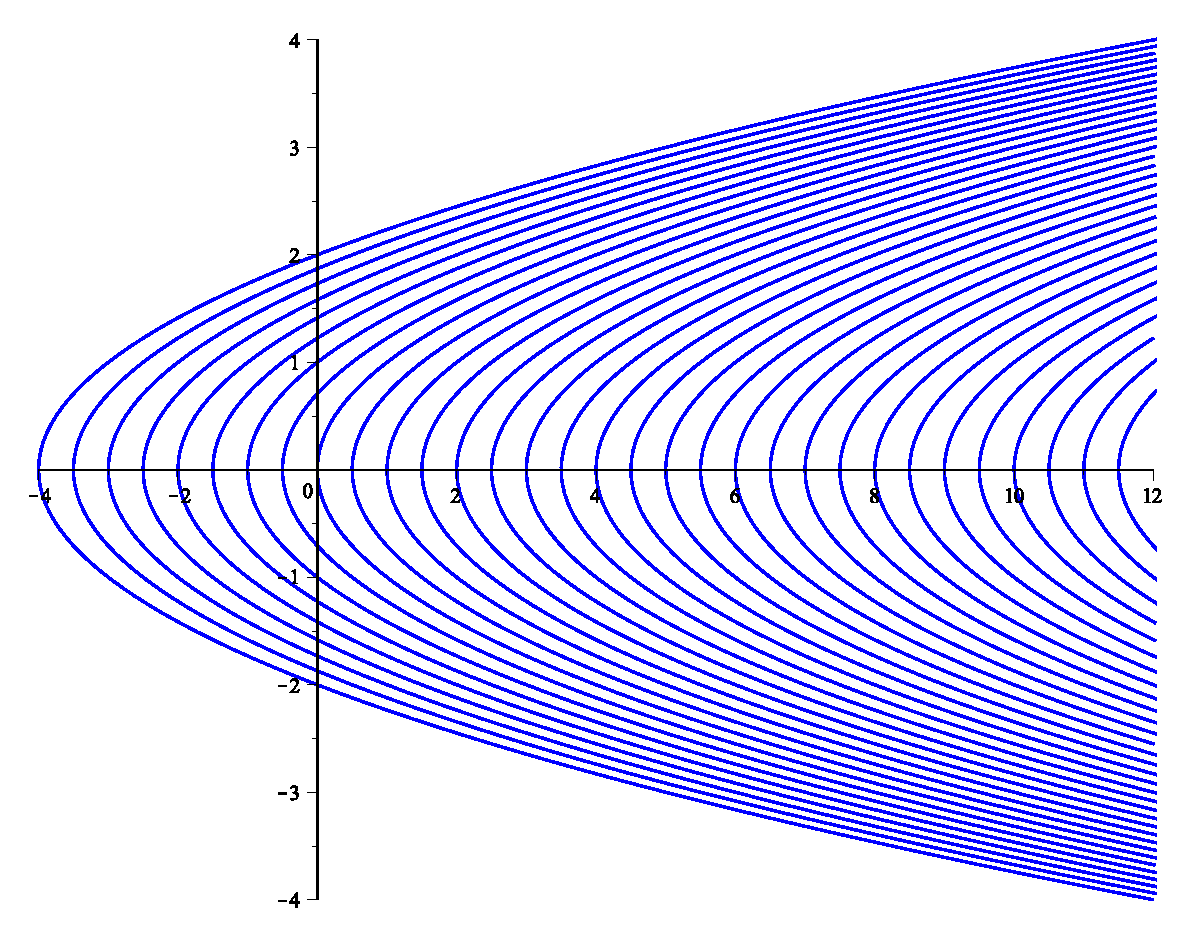
\includegraphics[width=100mm]{Figures/example_figure1.eps}
\caption{An example figure using encapsulated postscript (.eps) images.}
\label{fig:example_eps1}
\end{figure}
\end{spverbatim}
\begin{figure}[ht!]
\centering
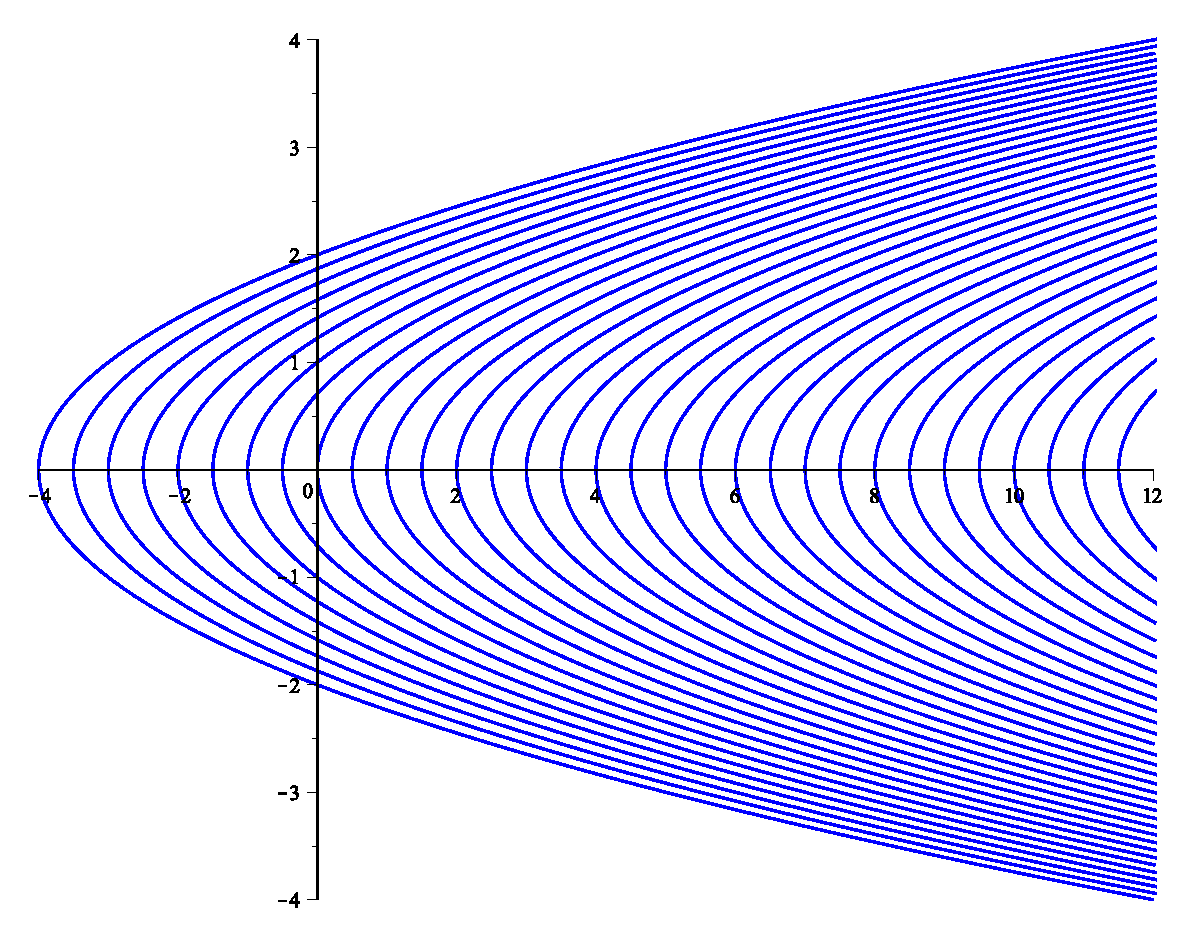
\includegraphics[width=100mm]{Figures/example_figure1.eps}
\caption{An example figure using encapsulated postscript (.eps) images.}
\label{fig:example_eps1}
\end{figure}
produces \autoref{fig:example_eps1}. Notice, when you zoom in, that no quality is lost from the image.

\subsection{Equation and figure numbering}
Equations, figures and theorems can sometimes be given the same numerical value.

For example, we may have the equation:
\begin{equation}\label{eqn:intdef}
\intbc[a][b]{\frac{f'(x)}{f(x)}}{x} = \log(f(b)) - \log(f(a))
\end{equation}
%
%\begin{equation}\label{indef}
%\intbc{\frac{f'(x)}{f(x)}}{x} = \log(f(x)) + C
%\end{equation}
%
and then the theorem:
\begin{theorem}\label{thm:thm}
I'm a theorem, I'm a theorem, I'm a theorem, I'm a theorem, I'm a theorem, I'm a theorem, I'm a theorem, I'm a theorem, I'm a theorem, I'm a theorem, a very nice theorem, I'm a theorem, I'm a theorem, I'm a theorem.
\end{theorem}
and also a figure, (\autoref{fig:example_eps2}).
\begin{figure}[ht!]
\centering
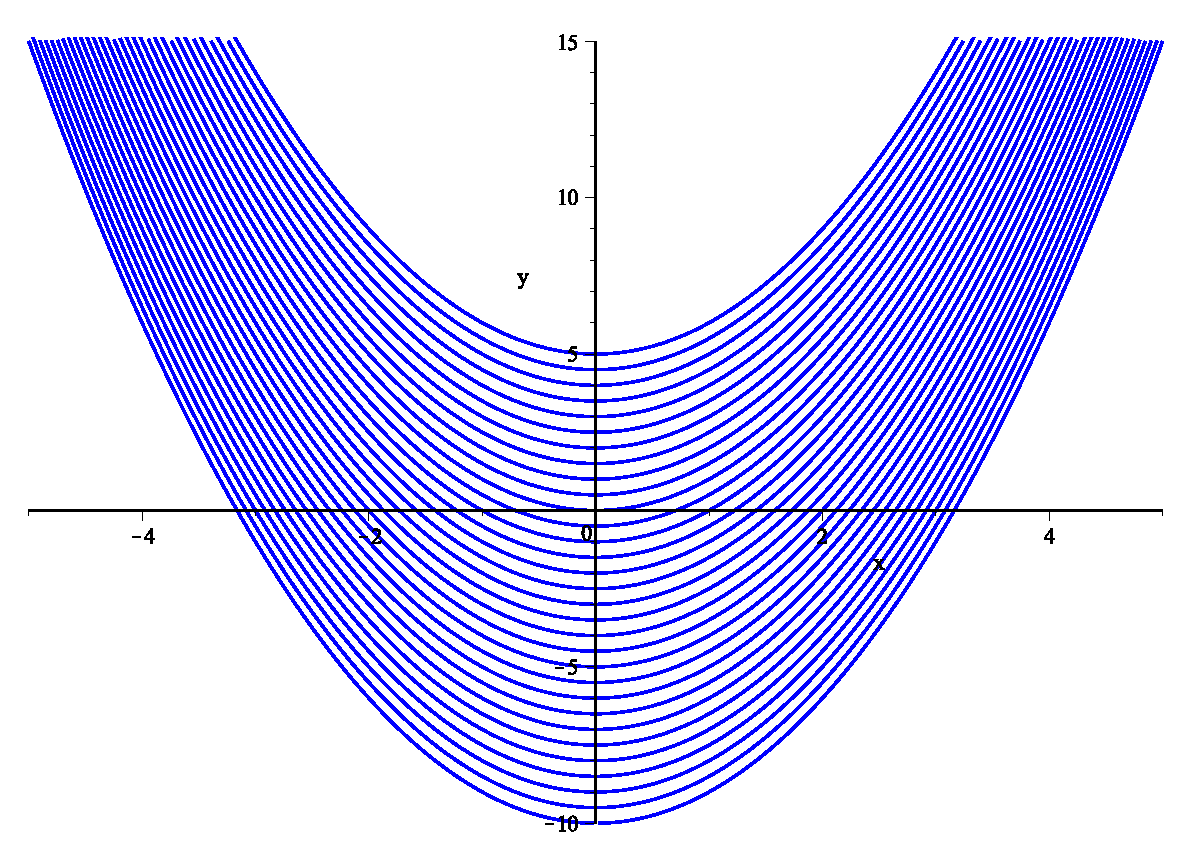
\includegraphics[width=100mm]{Figures/example_figure2.eps}
\caption{Another example figure using .eps images.}
\label{fig:example_eps2}
\end{figure}

\autoref{thm:thm}, \autoref{eqn:intdef} and \autoref{fig:mesh}, all have the same numerical value assigned to them.
When referencing, the \verb|\autoref{ }| command automatically affixes `Theorem', `Figure', or `Equation' in front of the numerical value, i.e.
\begin{spverbatim}
\autoref{thm:thm}, \autoref{eqn:intdef} and \autoref{fig:example_eps}, all have the same numerical value
\end{spverbatim}
produced the above statement.

For further details on theorem environments, see \autoref{ssec:thme}.
%\autoref{intdef} \%eqref{intdef}

\section{Nice things for applied mathematicians}
\subsection{Derivatives}
Custom commands for derivatives and partial derivatives can make your life much easier, and save you lots of time writing up, especially when writing out differential equations!

For example:
\begin{verbatim}
\[\D[2]{y}{x} - \lambda\D{y}{x} + \lambda^2 y = 0\]
\end{verbatim}
produces
\[\D[2]{y}{x} - \lambda\D{y}{x} + \lambda^2 y = 0\]
making full use of the ordinary derivative command, \verb|\D[]{}{}|. 

Similarly, a partial differential equation can be included using commands for partial derivatives \verb|\PD[]{}{}| and \verb|\PDxy{}{}{}|, like so:
\begin{spverbatim}
\[\PD[2]{\phi}{y} + xy \PD[2]{\phi}{x} - \phi \PDxy{\phi}{x}{y} + x^2\PD{\phi}{y} + 2\phi(x,y) = 0\]
\end{spverbatim}
produces
\[\PD[2]{\phi}{y} + xy \PD[2]{\phi}{x} - \phi \PDxy{\phi}{x}{y} + x^2\PD{\phi}{y} + 2\phi(x,y) = 0\]
If you don't like \verb|\D| or \verb|\PD| as the abbreviated commands - say you wanted to use \verb|\D| as a shortcut for \verb|\Delta| instead of an ordinary derivative - then these can easily be changed to anything of your choice by editing the \verb|ueathesis.sty| file.

For example changing 
\begin{spverbatim}
\newcommand{\D}[3][]{\frac{\text{d}^{#1} #2}{\text{d} #3^{#1}}}| 
\end{spverbatim}
to
\begin{spverbatim}
\newcommand{\Deriv}[3][]{\frac{\text{d}^{#1} #2}{\text{d} #3^{#1}}}
\end{spverbatim}
would mean writing \verb|\Deriv[2]{y}{x}| to express $\frac{\text{d}^2 y}{\text{d} x^2}$, instead of \verb|\D[2]{y}{x}|.
\subsection{Integrals}
Another useful custom command which we have included is \verb|\intbc[][]{}{}|. This allows you to quickly insert integrals, with optional limits.

For example:
\begin{spverbatim}
\[\intbc{\frac{1}{x^2+a^2}}{x} = \frac{1}{a}\tan^{-1}\left(\frac{x}{a}\right)+C\]
\end{spverbatim}
produces
\[\intbc{\frac{1}{x^2+a^2}}{x} = \frac{1}{a}\tan^{-1}\left(\frac{x}{a}\right)+C,\] 
then
\begin{spverbatim}
\[\intbc[1][2]{\frac{1}{x^2+1}}{x} = \tan^{-1}(2)-\tan^{-1}(1)\]
\end{spverbatim}
produces
\[\intbc[1][2]{\frac{1}{x^2+1}}{x} = \tan^{-1}(2)-\tan^{-1}(1).\]

Once again, if you aren't entirely happy with it being called \verb|\intbc| then you can change this in the \verb|ueathesis.sty| file.

\begin{remark}
This custom command uses the \verb|twoopt| package, which allows the use of two optional arguments in the new command. It works in exactly the same way, but \verb|\intbc| is defined using \verb|\newcommandtwoopt| instead of \verb|\newcommand|. 
\end{remark}

Alternatively, if you're working a lot with integrals with $[-\infty,\infty]$ limits, then the \verb|\intinf{}{}| command may be particularly useful - rather than writing \verb|-\infty| and \verb|\infty| into the \verb|\intbc| command each time. For example:
\begin{spverbatim}
\[\intinf{\sech^2(\xi)}{\xi} = 2\]
\end{spverbatim}
produces
\[\intinf{\sech^2(\xi)}{\xi} = 2.\]
The above integral also makes use of \verb|\sech| which isn't included in the standard \TeX{} distribution.

\subsection{Double and triple integrals}

\verb|ueathesis.sty| also has commands to handle multiple integrals. For instance, you can use the \verb|\dint| command for double integrals like so:

\begin{spverbatim}
\[\dint[]{0}{2\pi}{0}{a}{r}{r}{\theta} = \pi a^2\]
\[\dint[-r\sin(\theta)]{\pi}{2\pi}{0}{a}{r}{r}{\theta} = r a^2\]
\[\dint[]{}{}{}{}{r}{r}{\theta} = \frac{r^2\theta}{2}\]
\end{spverbatim}
gives
\[\dint[]{0}{2\pi}{0}{a}{r}{r}{\theta} = \pi a^2\]
\[\dint[-r\sin(\theta)]{\pi}{2\pi}{0}{a}{r}{r}{\theta} = r a^2\]
\[\dint[]{}{}{}{}{r}{r}{\theta} = \theta\left(\frac{r^2}{2}+c_1\right)+c_2\]

where the optional argument can be used for any functions that appear to the left of the latter integral sign.

As \LaTeX{} only accepts a maximum of nine arguments in a new command, it is difficult to write a similar command for triple integrals, which would require ten arguments. However, as the problem in typesetting triple integrals rests with the correct way to display the variables in the integrand, we have created the \verb|\tintd| and \verb|\tintl| commands. For example, the code

\begin{spverbatim}
\[\tintl[][]{0}{\pi}{0}{2\pi}{0}{a} \tintd{r^2\sin(\phi)}{r}{\theta}{\phi} = \frac{4\pi a^3}{3}\]
\end{spverbatim}


\[\tintl[][]{0}{\pi}{0}{2\pi}{0}{a}\tintd{r^2\sin(\phi)}{r}{\theta}{\phi} = \frac{4\pi a^3}{3}\]

where the \verb|\tintl| command handles the limits, and [optionally] any functions that may appear to the left of either of the latter two integral signs, and the \verb|\tintd| command takes care of typesetting the integrand $\tintd{r^2\sin(\phi)}{r}{\theta}{\phi}$.


\subsection{Summations and products}
This is a rather brief explanation for using the \verb|\sumtxt{}{}| and \verb|prodtxt{}{}| custom commands.

Summations and products in general are fairly straightforward to typeset, so no custom commands have been included. 
\begin{verbatim}
\[ \sum_{n=1}^{\infty} 2^{-n} =1 \]
\end{verbatim}
produces
\[\sum_{n=1}^{\infty} 2^{-n} =1,\]
and
\begin{verbatim}
%\[ \prod_{x=1}^{N} f(x) \]
\end{verbatim}
gives
\[ \prod_{x=1}^{N} f(x). \]
However, in text mode the limits appear to the right-hand side of the summation sign, like so: $\sum_{n=1}^{\infty} 2^{-n} =1$. Using the command \verb|\sumtxt{}{}|, where the first argument is your bottom limit and the second argument is the top limit, you can display summations in text in the traditional way.
\begin{verbatim}
This is what $\sumtxt{n=1}{\infty}$ looks like in text mode...
\end{verbatim}
This is what $\sumtxt{n=1}{\infty}$ looks like in text mode...
and similarly 
\begin{verbatim}
this is what $\prodtxt{x=1}{N}$ looks like in text mode.
\end{verbatim}
this is what $\prodtxt{x=1}{N}$ looks like in text mode.
\subsection{Really wide hat}
If your thesis involves a lot of numerical analysis, there is a good chance that you'll be working with Fourier transforms. 

A frequently used notation for displaying transformed functions is the \verb|\hat{}| notation. For example, $\hat{f}(k)$ may refer to the function $f(x)$ following a Fourier transform. While this is fairly straightforward, what if you would like to typeset the transformed version of, say:
\[\mc{S}(\tilde{\sigma}_S)\mc{S}(\tilde{\sigma}_{SS}) \]
 Using the \verb|\hat{}| command produces errors, as the expression is too large for the command parameters. The \verb|\widehat{}| command could be used:
\[ \widehat{\mc{S}(\tilde{\sigma}_S)\mc{S}(\tilde{\sigma}_{SS})}\]
but this doesn't look particularly great.

Never fear, \verb|\reallywidehat{}| is here! \\
Typing:
\begin{small}
\begin{spverbatim}
\[ \reallywidehat{\mc{S}(\tilde{\sigma}_S)\mc{S}(\tilde{\sigma}_{SS})} \]
\end{spverbatim}
\end{small}
(where \verb|\mc{S}| is a shortened command for \verb|\mathcal{S}|; see \autoref{tab:no}) produces
\[ \reallywidehat{\mc{S}(\tilde{\sigma}_S)\mc{S}(\tilde{\sigma}_{SS})} \]
which looks much better.




\section{Nice things for pure mathematicians}

\subsection{Theorem environments, numbering and referencing}{\label{ssec:thme}}

A notable feature of \verb|ueathesis.sty| is the ability to handle different kinds of theorem environments easily, with a structured count and referencing compatible with the \verb|hyperref| package. 

A list of the different theorem environments can be found in \autoref{tab:env}. 

\begin{table}[ht]
\renewcommand{\arraystretch}{1.5}
\centering
\begin{tabular}{lccl}
Environment / (alt) & Counted? & \verb|emph|? & Notes\\ \hline
\verb|lemma| / (\verb|lem|) & Y & Y & \\
\verb|proposition| / (\verb|prop|) & Y & Y & \\
\verb|theorem| / (\verb|thm|) & Y & Y & \\
\verb|corollary| / (\verb|cor|)  & Y & Y & \\
\verb|definition| / (\verb|defn|) & Y & N & \\
\verb|notation| / (\verb|not|) & Y & N & \\
\verb|example| / (\verb|ex|) & Y & N & \verb|examples| / (\verb|exs|) also defined\\
\verb|question| / (\verb|que|) & Y & Y & \\
\verb|conjecture| / (\verb|conj|) & Y & Y & \\
\verb|remark| / (\verb|rmk|) & N & N & \verb|remarks| / (\verb|rmks|) also defined\\
\verb|answer| & N & N & \\
\verb|claim| & N & N & \\
\verb|claimx| & N & N & \verb|x| = 1,2,3 \\
\verb|casex| & N & N & \verb|x| = 1,2,3 \\
\end{tabular}
\caption[Defined environments (and alternate option) in $\texttt{ueathesis.sty}$]{Defined environments (and alternate option) in $\texttt{ueathesis.sty}$. Counted? asks if it is counted along with theorems. $\texttt{emph}$? asks if text is italicised in the environment.}\label{tab:env}
\end{table}

You can use and reference these like normal environments; so \begin{verbatim}\begin{lemma}\label{lemma}...\end{lemma} By \autoref{lemma}...
\end{verbatim} will give \begin{lemma}\label{lemma} ... \end{lemma} By \autoref{lemma}...

Note here that the \verb|\autoref{lemma}| command displays the fact that the environment referenced was a lemma. Should you want to change this result to a \verb|proposition| environment, the reference in the text becomes ``Proposition...'', reflecting this change. Below is an example of some of the different environments mentioned in \autoref{tab:env} and what they look like. The verbatim of this exchange can be found in \autoref{app:verb}.

\begin{definition}\label{def:1} Dank = good.
\end{definition}

\begin{lemma}\label{lem:1} Dank lemma.
\end{lemma}

\begin{proof} Split into two cases. 
\begin{case1} Straightforward; it is dank by \autoref{def:1}.
\end{case1}

\begin{case2} By inspection, it is a lemma.
\end{case2}
We are done; this is a dank lemma. \end{proof}

\begin{example}\label{ex:1} For instance; dank.
\end{example}

\begin{remark} Note how dank \autoref{ex:1} is.
\end{remark}

\begin{theorem}\label{thm:1}
I'm a theorem I'm a theorem
\end{theorem}

\begin{proof} Using \autoref{def:1}, the proof follows from \autoref{lem:1}.
\end{proof}

\begin{corollary}\label{cor:1} \autoref{thm:1} is a dank theorem. \dne
\end{corollary}

\autoref{cor:1} is dank too. We can then ask:

\begin{question} Following \autoref{thm:1} and \autoref{cor:1}, are there any other dank theorems?
\end{question}

\subsection{Lists of defined operators, new and renewed commands}

Along with the theorem environments listed above, \verb|ueathesis.sty| contains lots of new commands to aid your typesetting of pure mathematics. These commands are detailed in \autoref{tab:no}, with the renewed commands detailed in \autoref{tab:renew}.

\begin{table}[ht!]
\renewcommand{\arraystretch}{1.5}
\centering
\begin{tabular}{llll}
Command & Argument? & Example & Display\\ \hline
\verb|\mb{}| & Mandatory & \verb|$\mb{R}\subseteq\mb{C}$| & $\mb{R}\subseteq\mb{C}$\\
\verb|\mc{}| & Mandatory & \verb|$\mc{R}\circ\mc{L}=\mc{D}$| & $\mc{R}\circ\mc{L}=\mc{D}$\\
\verb|\mf{}| & Mandatory & \verb|$\mf{p} + \mf{q}$| & $\mf{p} + \mf{q}$\\
\verb|\ms{}| & Mandatory & \verb|$\ms{C}$| & $\ms{C}$\\
\verb|\larr| & Optional & \verb|$G\larr[x] H$| & $G\larr[x] H$\\
\verb|\rarr| & Optional & \verb|$G\rarr[y] H$| & $G\rarr[y] H$\\
\verb|\Rarr| & Optional & \verb|$G\Rarr[z] H$| & $G\Rarr[z] H$\\
\verb|\from| & No & \verb|$G\from H$| & $G\from H$\\
\verb|\abs| & Mandatory & \verb|$\abs{x-a}$| & $\abs{x-a}$\\
\verb|\norm| & Mandatory & \verb|$\norm{x-a}$| & $\norm{x-a}$\\
\verb|\stl| & No & \verb|$\{x\stl x^2 = 1\}$| & $\{x\stl x^2 = 1\}$\\
\verb|\stc| & No & \verb|$\{x\stc x^2 = 1\}$| & $\{x\stc x^2 = 1\}$\\
\verb|\dne| & No & \verb|We are done. \dne| & We are done.\!\dne\\
\verb|\Aut| & No & \verb|$\Aut(\mb{C})$| & $\Aut(\mb{C})$
\end{tabular}
\caption{Some commands to assist with typsetting mathematics.}\label{tab:no}
\end{table}

In particular, the \verb|\Aut| command in \autoref{tab:no} is one of a family of declared mathematical operators in \verb|ueathesis.sty|. A list of all of them is given below; to use the command, add a backslash before the operator name you require (case sensitive).
\begin{align*}& \Aut,\coker,\dom,\End,\Ext,\Fix,\Gal,\Gel,\Hom,\im, \Ind \\ 
& \Int,\Lim,\Mod,\Ob,\Proj,\rad,\Stab,\Split,\Spec\end{align*}

Finally, \verb|ueathesis.sty| renews some commands that reflect the more common usage of some mathematical operators. \autoref{tab:renew} details the changes made. You can revert back to the `before' setting by commenting out the relevant \verb|let| or \verb|\renewcommand| commands in \verb|% 5.12 Miscellaneous| of \verb|ueathesis.sty|.

\begin{table}[ht!]
\renewcommand{\arraystretch}{1.5}
\centering
\begin{tabular}{llll}
Command & Before & After & Example\\ \hline
\verb|\emptyset| & $\oldemptyset$ & $\emptyset$ & $A\cap B = \varnothing$\\
\verb|\Re| & $\oldRe$ & $\Re$ & $\mathrm{Re}(z) = 4$\\
\verb|\Im| & $\oldIm$ & $\Im$ & $\mathrm{Im}(z) = 4$
\end{tabular}
\caption{Renewed commands in \texttt{ueathesis.sty}}\label{tab:renew}
\end{table}

\begin{remark} The reason for the amount of \verb|let| commands in this portion of the style file, rather than a relatively straightforward usage of \verb|renewcommand|, was purely to produce this table.
\end{remark}

\section{Nice things for engineers}

With thanks to Francesco Parente for bringing \citep{beccari1997typesetting} to our attention.

\subsection{Handling SI units}

There is an established convention when typesetting SI units, as mentioned in the SI Brochure. Typically, units must be in an upright type, with a `thin space' between the quantity and the unit.

The command \verb|\unit| provides this correct typesetting for SI units. For instance, the command \begin{verbatim}\[ g = 9.81\unit{m/s^2} \]
\end{verbatim}
gives
\[ g = 9.81\unit{m/s^2} \]

Furthermore, \autoref{tab:si} defines some commands for commonly used scientific notation.

\begin{table}
\renewcommand{\arraystretch}{1.5}
\centering
\begin{tabular}{lllll}
Command & Argument? & Meaning & Example & Display\\ \hline
\verb|\angs| & No & Angstrom & \verb|$10\unit{\angs}$| & $10\unit{\angs}$\\
\verb|\degree[]| & Optional & Degrees & \verb|$30\unit{\degree[C]}$| & $30\unit{\degree[C]}$ \\
& & & \verb|$90\unit{\degree}$| & $90\unit{\degree}\quad$\\
\verb|\ohm| & No & Ohms & \verb|$10\unit{m\ohm}$| & $10\unit{m\ohm}$\\
\verb|\micro| & No & micro & \verb|$10\unit{\micro g}$| & $10\unit{\micro g}$\\
\end{tabular}
\caption{Some commands to assist with typsetting SI units.}\label{tab:si}
\end{table}

\subsection{Properly typeset numerical constants}
To avoid confusion with mathematical variables, numerical constants should also be typeset correctly. One of the most commonly used numerical constants is Euler's constant, \eu, the base of natural logarithms. In \verb|ueathesis.sty|, this has been given the command \verb|\eu|.
\begin{spverbatim}
Euler's constant, \eu{} can be added to my thesis. I can also include it in `math mode,' $\eu=2.718\ldots$
\end{spverbatim}
Euler's constant, \eu{} can be added to my thesis. I can also include it in `math mode,' $\eu=2.718\ldots$.
\begin{remark}
When not in math mode, the use of $\{\}$ following the \verb|\eu| ensures a space between \eu{} and the text that follows.
\end{remark}
Working with complex numbers? Remember to typeset your imaginary units correctly. \autoref{tab:imag} details the correct use of imaginary units \iu{} and \ju{}, complete with examples.
\begin{table}[ht!]
\renewcommand{\arraystretch}{1.5}
\centering
\begin{tabular}{lllll}
Command & Argument? & Meaning & Example & Display\\ \hline
\verb|\iu{}| & Only in & Imag. unit $\iu=\sqrt{-1}$ & \verb|$3+4\iu$| & $3+4\iu$\\
 & text &  (for civilised people) & & \\
\verb|\ju{}| & Only in & Imag. unit $\ju=\sqrt{-1}$ & \verb|\ju{}| & \ju{}  \\
 & text &  (for savages) &  & \\
\end{tabular}
\caption{Some commands to assist with correctly typsetting imaginary units.}\label{tab:imag}
\end{table}

While this text has included three common numerical constants, \eu{}, \iu{}, and \ju{}, you are of course free to add your own to the \verb|ueathesis.sty| file. The first three are included under \verb|%5.9 Engineering , science and technology|, as follows:
\begin{spverbatim}
\providecommand*{\eu}{\ensuremath{\mathrm{e}}}
\end{spverbatim}
To include your own you can insert
\begin{spverbatim}
\providecommand*{\commandname]}{\ensuremath{\mathrm{constant}}}
\end{spverbatim}
changing the values of \verb|commandname| and \verb|constant| as necessary.

\begin{remark}
It may be that your new command name already exists as a \LaTeX{} command. Here, the use of \verb|providecommand| ensures that there are no errors when compiling with your new command. If you are certain that your new command name is \emph{not} a pre-existing command, you can use \verb|newcommand| instead of \verb|providecommand|.
\end{remark}
\subsection{Superscripts and subscripts that don't italicise text}
Standard \TeX{} requires you to use ‘math mode’ to use subscripts and superscripts within text. For example, if you wished to abbreviate the words \emph{first}, \emph{second}, \emph{third} and \emph{fourth}, you might put:
\begin{verbatim}
1$^{st}$, 2$^{nd}$, 3$^{rd}$ and 4$^{th}$
\end{verbatim}
which would produce: 1$^{st}$, 2$^{nd}$, 3$^{rd}$ and 4$^{th}$. The problem here is that the \emph{st}, \emph{nd}, \emph{rd} and \emph{th} are all typeset in ‘math mode.’ 

Likewise, if you're typing equations and wish to define values $x\ped{a}$, $x\ped{b}$ and $x\ped{c}$, say, then using the standard subscript command \verb|_{ }|, would produce $x_a$, $x_b$ and $x_c$. Again, the \emph{a}, \emph{b} and \emph{c} have all been typeset in ‘math mode.’

A workaround for this could be to write:
\begin{spverbatim}
1$^{\text{st}}$, 2$^{\text{nd}}$, 3$^{\text{rd}}$, 4$^{\text{th}}$
\end{spverbatim}
or 
\begin{spverbatim}
$x_{\text{a}}$, $x_{\text{b}}$, $x_{\text{c}}$
\end{spverbatim}
which give 1$^{\text{st}}$, 2$^{\text{nd}}$, 3$^{\text{rd}}$, 4$^{\text{th}}$ and $x_{\text{a}}$, $x_{\text{b}}$ and $x_{\text{c}}$.

These workarounds do work, but can become overly complicated and take a long time to write up each time. 

To combat this, we've included the custom commands \verb|\ped| and \verb|\ap| for subscripts and superscripts, respectively. For example, writing:
\begin{spverbatim}
$x\ped{a}$, $x\ped{b}$, and $x\ped{c}$
\end{spverbatim}
yields $x\ped{a}$, $x\ped{b}$, and $x\ped{c}$. Also,
\begin{spverbatim}
1\ap{st}, 2\ap{nd}, 3\ap{rd} and 4\ap{th}
\end{spverbatim}
returns 1\ap{st}, 2\ap{nd}, 3\ap{rd} and 4\ap{th}. Notice how the commands can be used freely in both ‘math mode’ and ‘text mode’ without error. 

Finally, as with any of the custom commands defined here, if you don't like the commands \verb|ap| and \verb|ped|, then these can be changed by editing the \verb|ueathesis.sty| file. 


\chapter{Body text example}

% ONLY COMMENT IN IF USING ueathesis.cls AS DOCUMENT CLASS
\begin{synopsis}
\noindent This chapter is filler text in order to examine how large blocks of text look and feel in the document. We feel that the synopsis environment is best used with a centrally aligned chapter heading. 
\end{synopsis}

Here is some text\footnote{with a footnote}.

The footnote has been produced using the \verb|\footnote{ }| command, like so:
\begin{verbatim}
Here is some text\footnote{with a footnote}.

\end{verbatim}

\section{Lorem ipsum}
\lipsum[1-6]
\section{Nullam eleifend}
\lipsum[7-12]